% Options for packages loaded elsewhere
\PassOptionsToPackage{unicode}{hyperref}
\PassOptionsToPackage{hyphens}{url}
\PassOptionsToPackage{dvipsnames,svgnames,x11names}{xcolor}
%
\documentclass[
  letterpaper,
  DIV=11,
  numbers=noendperiod]{scrartcl}

\usepackage{amsmath,amssymb}
\usepackage{iftex}
\ifPDFTeX
  \usepackage[T1]{fontenc}
  \usepackage[utf8]{inputenc}
  \usepackage{textcomp} % provide euro and other symbols
\else % if luatex or xetex
  \usepackage{unicode-math}
  \defaultfontfeatures{Scale=MatchLowercase}
  \defaultfontfeatures[\rmfamily]{Ligatures=TeX,Scale=1}
\fi
\usepackage{lmodern}
\ifPDFTeX\else  
    % xetex/luatex font selection
\fi
% Use upquote if available, for straight quotes in verbatim environments
\IfFileExists{upquote.sty}{\usepackage{upquote}}{}
\IfFileExists{microtype.sty}{% use microtype if available
  \usepackage[]{microtype}
  \UseMicrotypeSet[protrusion]{basicmath} % disable protrusion for tt fonts
}{}
\makeatletter
\@ifundefined{KOMAClassName}{% if non-KOMA class
  \IfFileExists{parskip.sty}{%
    \usepackage{parskip}
  }{% else
    \setlength{\parindent}{0pt}
    \setlength{\parskip}{6pt plus 2pt minus 1pt}}
}{% if KOMA class
  \KOMAoptions{parskip=half}}
\makeatother
\usepackage{xcolor}
\setlength{\emergencystretch}{3em} % prevent overfull lines
\setcounter{secnumdepth}{-\maxdimen} % remove section numbering
% Make \paragraph and \subparagraph free-standing
\ifx\paragraph\undefined\else
  \let\oldparagraph\paragraph
  \renewcommand{\paragraph}[1]{\oldparagraph{#1}\mbox{}}
\fi
\ifx\subparagraph\undefined\else
  \let\oldsubparagraph\subparagraph
  \renewcommand{\subparagraph}[1]{\oldsubparagraph{#1}\mbox{}}
\fi

\usepackage{color}
\usepackage{fancyvrb}
\newcommand{\VerbBar}{|}
\newcommand{\VERB}{\Verb[commandchars=\\\{\}]}
\DefineVerbatimEnvironment{Highlighting}{Verbatim}{commandchars=\\\{\}}
% Add ',fontsize=\small' for more characters per line
\usepackage{framed}
\definecolor{shadecolor}{RGB}{241,243,245}
\newenvironment{Shaded}{\begin{snugshade}}{\end{snugshade}}
\newcommand{\AlertTok}[1]{\textcolor[rgb]{0.68,0.00,0.00}{#1}}
\newcommand{\AnnotationTok}[1]{\textcolor[rgb]{0.37,0.37,0.37}{#1}}
\newcommand{\AttributeTok}[1]{\textcolor[rgb]{0.40,0.45,0.13}{#1}}
\newcommand{\BaseNTok}[1]{\textcolor[rgb]{0.68,0.00,0.00}{#1}}
\newcommand{\BuiltInTok}[1]{\textcolor[rgb]{0.00,0.23,0.31}{#1}}
\newcommand{\CharTok}[1]{\textcolor[rgb]{0.13,0.47,0.30}{#1}}
\newcommand{\CommentTok}[1]{\textcolor[rgb]{0.37,0.37,0.37}{#1}}
\newcommand{\CommentVarTok}[1]{\textcolor[rgb]{0.37,0.37,0.37}{\textit{#1}}}
\newcommand{\ConstantTok}[1]{\textcolor[rgb]{0.56,0.35,0.01}{#1}}
\newcommand{\ControlFlowTok}[1]{\textcolor[rgb]{0.00,0.23,0.31}{#1}}
\newcommand{\DataTypeTok}[1]{\textcolor[rgb]{0.68,0.00,0.00}{#1}}
\newcommand{\DecValTok}[1]{\textcolor[rgb]{0.68,0.00,0.00}{#1}}
\newcommand{\DocumentationTok}[1]{\textcolor[rgb]{0.37,0.37,0.37}{\textit{#1}}}
\newcommand{\ErrorTok}[1]{\textcolor[rgb]{0.68,0.00,0.00}{#1}}
\newcommand{\ExtensionTok}[1]{\textcolor[rgb]{0.00,0.23,0.31}{#1}}
\newcommand{\FloatTok}[1]{\textcolor[rgb]{0.68,0.00,0.00}{#1}}
\newcommand{\FunctionTok}[1]{\textcolor[rgb]{0.28,0.35,0.67}{#1}}
\newcommand{\ImportTok}[1]{\textcolor[rgb]{0.00,0.46,0.62}{#1}}
\newcommand{\InformationTok}[1]{\textcolor[rgb]{0.37,0.37,0.37}{#1}}
\newcommand{\KeywordTok}[1]{\textcolor[rgb]{0.00,0.23,0.31}{#1}}
\newcommand{\NormalTok}[1]{\textcolor[rgb]{0.00,0.23,0.31}{#1}}
\newcommand{\OperatorTok}[1]{\textcolor[rgb]{0.37,0.37,0.37}{#1}}
\newcommand{\OtherTok}[1]{\textcolor[rgb]{0.00,0.23,0.31}{#1}}
\newcommand{\PreprocessorTok}[1]{\textcolor[rgb]{0.68,0.00,0.00}{#1}}
\newcommand{\RegionMarkerTok}[1]{\textcolor[rgb]{0.00,0.23,0.31}{#1}}
\newcommand{\SpecialCharTok}[1]{\textcolor[rgb]{0.37,0.37,0.37}{#1}}
\newcommand{\SpecialStringTok}[1]{\textcolor[rgb]{0.13,0.47,0.30}{#1}}
\newcommand{\StringTok}[1]{\textcolor[rgb]{0.13,0.47,0.30}{#1}}
\newcommand{\VariableTok}[1]{\textcolor[rgb]{0.07,0.07,0.07}{#1}}
\newcommand{\VerbatimStringTok}[1]{\textcolor[rgb]{0.13,0.47,0.30}{#1}}
\newcommand{\WarningTok}[1]{\textcolor[rgb]{0.37,0.37,0.37}{\textit{#1}}}

\providecommand{\tightlist}{%
  \setlength{\itemsep}{0pt}\setlength{\parskip}{0pt}}\usepackage{longtable,booktabs,array}
\usepackage{calc} % for calculating minipage widths
% Correct order of tables after \paragraph or \subparagraph
\usepackage{etoolbox}
\makeatletter
\patchcmd\longtable{\par}{\if@noskipsec\mbox{}\fi\par}{}{}
\makeatother
% Allow footnotes in longtable head/foot
\IfFileExists{footnotehyper.sty}{\usepackage{footnotehyper}}{\usepackage{footnote}}
\makesavenoteenv{longtable}
\usepackage{graphicx}
\makeatletter
\def\maxwidth{\ifdim\Gin@nat@width>\linewidth\linewidth\else\Gin@nat@width\fi}
\def\maxheight{\ifdim\Gin@nat@height>\textheight\textheight\else\Gin@nat@height\fi}
\makeatother
% Scale images if necessary, so that they will not overflow the page
% margins by default, and it is still possible to overwrite the defaults
% using explicit options in \includegraphics[width, height, ...]{}
\setkeys{Gin}{width=\maxwidth,height=\maxheight,keepaspectratio}
% Set default figure placement to htbp
\makeatletter
\def\fps@figure{htbp}
\makeatother

\usepackage{fvextra}
\DefineVerbatimEnvironment{Highlighting}{Verbatim}{breaklines,commandchars=\\\{\}}
\DefineVerbatimEnvironment{OutputCode}{Verbatim}{breaklines,commandchars=\\\{\}}
\KOMAoption{captions}{tableheading}
\makeatletter
\makeatother
\makeatletter
\makeatother
\makeatletter
\@ifpackageloaded{caption}{}{\usepackage{caption}}
\AtBeginDocument{%
\ifdefined\contentsname
  \renewcommand*\contentsname{Table of contents}
\else
  \newcommand\contentsname{Table of contents}
\fi
\ifdefined\listfigurename
  \renewcommand*\listfigurename{List of Figures}
\else
  \newcommand\listfigurename{List of Figures}
\fi
\ifdefined\listtablename
  \renewcommand*\listtablename{List of Tables}
\else
  \newcommand\listtablename{List of Tables}
\fi
\ifdefined\figurename
  \renewcommand*\figurename{Figure}
\else
  \newcommand\figurename{Figure}
\fi
\ifdefined\tablename
  \renewcommand*\tablename{Table}
\else
  \newcommand\tablename{Table}
\fi
}
\@ifpackageloaded{float}{}{\usepackage{float}}
\floatstyle{ruled}
\@ifundefined{c@chapter}{\newfloat{codelisting}{h}{lop}}{\newfloat{codelisting}{h}{lop}[chapter]}
\floatname{codelisting}{Listing}
\newcommand*\listoflistings{\listof{codelisting}{List of Listings}}
\makeatother
\makeatletter
\@ifpackageloaded{caption}{}{\usepackage{caption}}
\@ifpackageloaded{subcaption}{}{\usepackage{subcaption}}
\makeatother
\makeatletter
\@ifpackageloaded{tcolorbox}{}{\usepackage[skins,breakable]{tcolorbox}}
\makeatother
\makeatletter
\@ifundefined{shadecolor}{\definecolor{shadecolor}{rgb}{.97, .97, .97}}
\makeatother
\makeatletter
\makeatother
\makeatletter
\makeatother
\ifLuaTeX
  \usepackage{selnolig}  % disable illegal ligatures
\fi
\IfFileExists{bookmark.sty}{\usepackage{bookmark}}{\usepackage{hyperref}}
\IfFileExists{xurl.sty}{\usepackage{xurl}}{} % add URL line breaks if available
\urlstyle{same} % disable monospaced font for URLs
\hypersetup{
  pdftitle={BST 270: Individual Project},
  pdfauthor={Nikhil Vytla},
  colorlinks=true,
  linkcolor={blue},
  filecolor={Maroon},
  citecolor={Blue},
  urlcolor={Blue},
  pdfcreator={LaTeX via pandoc}}

\title{BST 270: Individual Project}
\usepackage{etoolbox}
\makeatletter
\providecommand{\subtitle}[1]{% add subtitle to \maketitle
  \apptocmd{\@title}{\par {\large #1 \par}}{}{}
}
\makeatother
\subtitle{Reproducible Data Science: Hate Crimes (FiveThirtyEight)}
\author{Nikhil Vytla}
\date{}

\begin{document}
\maketitle
\ifdefined\Shaded\renewenvironment{Shaded}{\begin{tcolorbox}[interior hidden, breakable, boxrule=0pt, frame hidden, sharp corners, enhanced, borderline west={3pt}{0pt}{shadecolor}]}{\end{tcolorbox}}\fi

\hypertarget{introduction}{%
\subsection{Introduction}\label{introduction}}

The following notebook aims to satisfy the requirements for the
individual project component of BST 270: Reproducible Data Science,
taken Winter 2024.

\hypertarget{motivations-and-reproducibility}{%
\paragraph{Motivations and
Reproducibility}\label{motivations-and-reproducibility}}

My aim is to reproduce two figures from FiveThirtyEight's
\href{https://fivethirtyeight.com/features/higher-rates-of-hate-crimes-are-tied-to-income-inequality/}{Higher
Rates Of Hate Crimes Are Tied To Income Inequality}.

Specifically, I aim to reproduce the two provided geographic plots on
pre- and post-election hate crime rates. I will utilize the provided
dataset based on FBI and SPLC survey data on hate crimes, located at
\texttt{../data/hate\_crimes.csv}.

\hypertarget{setup}{%
\subsection{Setup}\label{setup}}

First, we load our required packages and required dataset. We utilize
the \texttt{usmap} library to easily plot U.S.-based geographic data,
which our CSV file is compatible with. We utilize the \texttt{ggplot2}
library to add additional graphical customization to our plot
(e.g.~titles, custom scales, fills, colors, etc.).

We directly download and read the CSV file from FiveThirtyEight's
official GitHub repository:
\href{https://github.com/fivethirtyeight/data/tree/master/hate-crimes}{fivethirtyeight/data/hate-crimes}.

\begin{quote}
NOTE: Alternatively, there is an
\href{https://cran.r-project.org/web/packages/fivethirtyeight/vignettes/fivethirtyeight.html}{unofficially
published R package named fivethirtyeight} that provides easy access to
FiveThirtyEight's GitHub-published datasets.
\end{quote}

\begin{Shaded}
\begin{Highlighting}[]
\FunctionTok{library}\NormalTok{(usmap)}
\FunctionTok{library}\NormalTok{(ggplot2)}

\NormalTok{hate\_crimes\_data }\OtherTok{\textless{}{-}} \FunctionTok{read.csv}\NormalTok{(}\StringTok{"https://raw.githubusercontent.com/fivethirtyeight/data/master/hate{-}crimes/hate\_crimes.csv"}\NormalTok{)}
\FunctionTok{write.csv}\NormalTok{(hate\_crimes\_data, }\AttributeTok{file=}\StringTok{\textquotesingle{}../data/hate\_crimes.csv\textquotesingle{}}\NormalTok{, }\AttributeTok{quote=}\ConstantTok{FALSE}\NormalTok{, }\AttributeTok{row.names =} \ConstantTok{FALSE}\NormalTok{)}
\end{Highlighting}
\end{Shaded}

\hypertarget{reproducing-plots}{%
\subsection{Reproducing Plots}\label{reproducing-plots}}

\hypertarget{figure-1-plot-pre-election-hate-crime-rates}{%
\subsubsection{Figure 1: Plot pre-election hate crime
rates}\label{figure-1-plot-pre-election-hate-crime-rates}}

The first figure plots pre-election hate crime rates per 100,000
residents between 2010-2015 per data sourced from the FBI Uniform Crime
Reporting Program.

\begin{Shaded}
\begin{Highlighting}[]
\FunctionTok{plot\_usmap}\NormalTok{(}\AttributeTok{data =}\NormalTok{ hate\_crimes\_data, }\AttributeTok{values =} \StringTok{"avg\_hatecrimes\_per\_100k\_fbi"}\NormalTok{, }\AttributeTok{color =} \StringTok{"grey"}\NormalTok{) }\SpecialCharTok{+} 
  \FunctionTok{scale\_fill\_continuous}\NormalTok{(}\AttributeTok{name =} \StringTok{"Average annual hate crimes per 100,000 residents, 2010{-}15"}\NormalTok{, }\AttributeTok{label =}\NormalTok{ scales}\SpecialCharTok{::}\NormalTok{comma, }\AttributeTok{low =} \StringTok{"white"}\NormalTok{, }\AttributeTok{high =} \StringTok{"\#ed4900"}\NormalTok{) }\SpecialCharTok{+} 
  \FunctionTok{theme}\NormalTok{(}\AttributeTok{legend.position =} \StringTok{"top"}\NormalTok{) }\SpecialCharTok{+}
  \FunctionTok{labs}\NormalTok{(}\AttributeTok{title =} \StringTok{"Pre{-}Election Hate Crime Rates"}\NormalTok{,}
       \AttributeTok{subtitle =} \StringTok{"Source: FBI Uniform Crime Reporting Program (UCR)"}\NormalTok{)}
\end{Highlighting}
\end{Shaded}

\begin{figure}[H]

{\centering 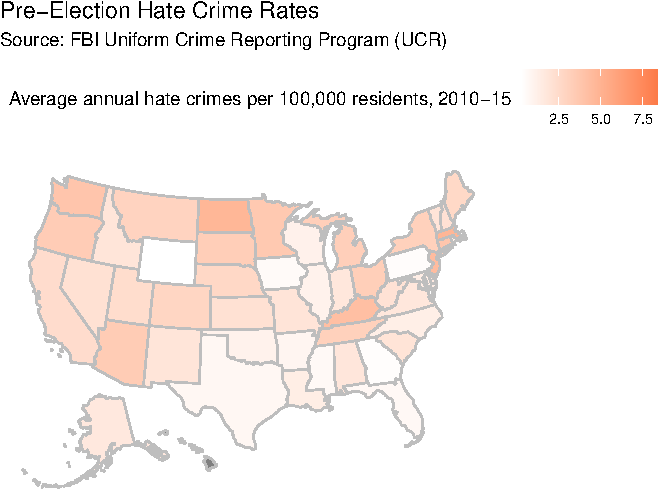
\includegraphics{hate_crimes_reproduction_files/figure-pdf/pre-election-hate-crimes-1.pdf}

}

\end{figure}

\hypertarget{figure-2-plot-post-election-hate-incidence-rates}{%
\subsubsection{Figure 2: Plot post-election hate incidence
rates}\label{figure-2-plot-post-election-hate-incidence-rates}}

The second figure plots post-election hate incidence rates per 100,000
residents in the 10 days after November 8, 2016, as reported by SPLC.

\begin{Shaded}
\begin{Highlighting}[]
\FunctionTok{plot\_usmap}\NormalTok{(}\AttributeTok{data =}\NormalTok{ hate\_crimes\_data, }\AttributeTok{values =} \StringTok{"hate\_crimes\_per\_100k\_splc"}\NormalTok{, }\AttributeTok{color =} \StringTok{"grey"}\NormalTok{) }\SpecialCharTok{+} 
  \FunctionTok{scale\_fill\_binned}\NormalTok{(}\AttributeTok{name =} \StringTok{"Hate Incidents per 100,000 residents in the 10 days after Nov. 8, 2016"}\NormalTok{, }\AttributeTok{label =}\NormalTok{ scales}\SpecialCharTok{::}\NormalTok{comma, }\AttributeTok{low =} \StringTok{"\#ffffff"}\NormalTok{, }\AttributeTok{high =} \StringTok{"\#00b37b"}\NormalTok{) }\SpecialCharTok{+} 
  \FunctionTok{theme}\NormalTok{(}\AttributeTok{legend.position =} \StringTok{"top"}\NormalTok{) }\SpecialCharTok{+}
  \FunctionTok{labs}\NormalTok{(}\AttributeTok{title =} \StringTok{"Post{-}Election Hate Incidence Rates"}\NormalTok{,}
       \AttributeTok{subtitle =} \StringTok{"Source: Southern Poverty Law Center (SPLC)"}\NormalTok{)}
\end{Highlighting}
\end{Shaded}

\begin{figure}[H]

{\centering 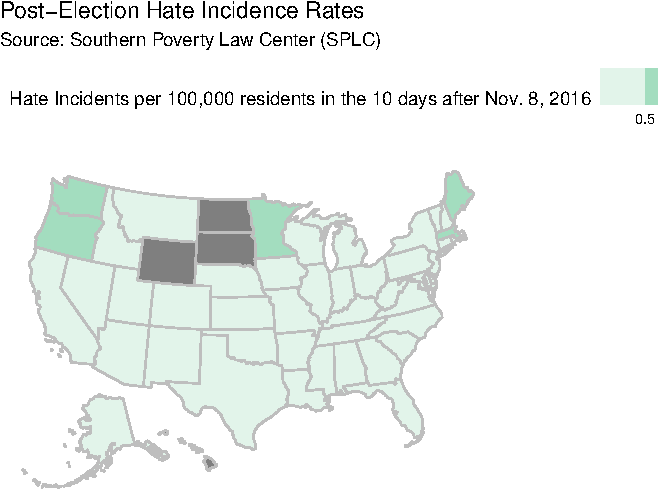
\includegraphics{hate_crimes_reproduction_files/figure-pdf/post-election-hate-incidences-1.pdf}

}

\end{figure}

\hypertarget{limitations-and-biases}{%
\subsection{Limitations and Biases}\label{limitations-and-biases}}

The author mentions the following biases in the original data sources
used:

\begin{quote}
``The federal government doesn't track hate crimes systematically
(agencies report to the FBI voluntarily), and the Southern Poverty Law
Center uses media accounts and people's self-reports to assess the
situation. Moreover, FBI hate crimes data for 2016 won't be released for
another several months, and the Southern Poverty Law Center didn't
collect data before the 2016 election. However, both data sources are
publicly available and easy to navigate, which means they're some of the
best we have.

But they also have biases baked in.

The FBI \href{https://ucr.fbi.gov/}{Uniform Crime Reporting Program}
collects hate crime data from law enforcement agencies. But because the
data is submitted voluntarily, it's unclear how comprehensive the data
set is. We don't have data from Hawaii, for instance. Moreover, the UCR
Program collects data on only prosecutable hate \emph{crimes}, which
make up a fraction of hate \emph{incidents} (which includes
non-prosecutable offenses, such as circulation of
\href{http://www.scpr.org/news/2016/11/16/66172/ucla-quickly-removes-white-nationalist-fliers-from/}{white
nationalist recruitment materials} on college campuses).

On the other hand, the Southern Poverty Law Center data --- which comes
from a combination of curated media accounts and self-reported form
entries --- includes both hate \emph{crimes} and non-prosecutable hate
\emph{incidents}. Moreover, heightened news coverage of hate incidents
after the election may have encouraged people to report incidents that
they would not have otherwise reported. This is called awareness bias
--- a trend that is well-established in epidemiology,
\href{http://journals.lww.com/epidem/Abstract/2000/03000/An_Exploration_of_Awareness_Bias_in_Two.20.aspx}{environmental
health} and other fields of research that frequently use self-reported
data.''
\end{quote}



\end{document}
